\usetheme{uclouvain}	

% THEME OPTIONS
% =============

% By default the beamer class adds navigation buttons. To remove them one can place
\beamertemplatenavigationsymbolsempty

% optional title page image
%\titlegraphic{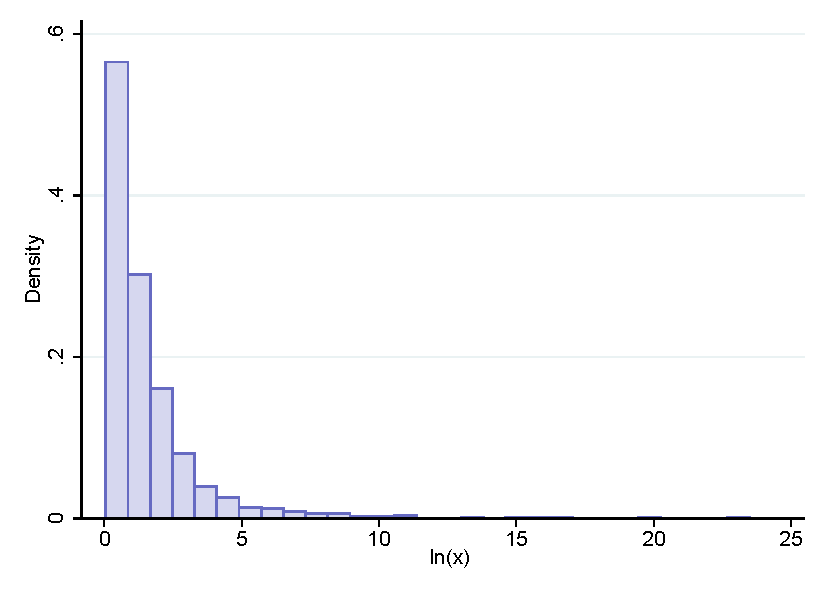
\includegraphics[width=0.4\textwidth]{example_figure.pdf}} 

% TODO Theme options:
% - nonav
% - nofootline
% - nosectiontoc
% - nosectiontitle
%
% TODO Frame options:
% - focus_light
% - focus_dark


% Select the font for the text
%\usepackage{lmodern}
\usepackage{biolinum}


\usepackage[T1]{fontenc}
\usepackage[utf8]{inputenc}
\usepackage[english]{babel}

\usepackage{amsfonts}
\usepackage{amssymb}

% math font with serifs, delete to make it sans-serif
\usefonttheme[onlymath]{serif}			

\usepackage{tikz}
\usetikzlibrary{shapes,shadows,arrows,backgrounds,mindmap,decorations.pathreplacing,positioning}

\usepackage{hyperref}
\hypersetup{
    % bookmarksnumbered,
    % bookmarks=true,         % show bookmarks bar?
    unicode=true,          % non-Latin characters in Acrobat’s bookmarks
    % pdftoolbar=true,        % show Acrobat’s toolbar?
    % pdfmenubar=true,        % show Acrobat’s menu?
    % pdffitwindow=true,      % window fit to page when opened
    % pdfstartview={FitH},    % fits the width of the page to the window
    % pdftitle={My title},    % title
    % pdfauthor={Author},     % author
    % pdfsubject={Subject},   % subject of the document
    % pdfcreator={Creator},   % creator of the document
    % pdfproducer={Producer}, % producer of the document
    % pdfkeywords={keyword1} {key2} {key3}, % list of keywords
    % pdfnewwindow=true,      % links in new window
    % colorlinks=true,       % false: boxed links; true: colored links
    % linkcolor=black,          % color of internal links
    % citecolor=black,        % color of links to bibliography
    % filecolor=black,      % color of file links
    % urlcolor=black,           % color of external links
    % hidelinks=true
}



